\documentclass[
  man,
  longtable,
  nolmodern,
  notxfonts,
  notimes,
  colorlinks=true,linkcolor=blue,citecolor=blue,urlcolor=blue]{apa7}

\usepackage{amsmath}
\usepackage{amssymb}




\RequirePackage{longtable}
\RequirePackage{threeparttablex}

\makeatletter
\renewcommand{\paragraph}{\@startsection{paragraph}{4}{\parindent}%
	{0\baselineskip \@plus 0.2ex \@minus 0.2ex}%
	{-.5em}%
	{\normalfont\normalsize\bfseries\typesectitle}}

\renewcommand{\subparagraph}[1]{\@startsection{subparagraph}{5}{0.5em}%
	{0\baselineskip \@plus 0.2ex \@minus 0.2ex}%
	{-\z@\relax}%
	{\normalfont\normalsize\bfseries\itshape\hspace{\parindent}{#1}\textit{\addperi}}{\relax}}
\makeatother




\usepackage{longtable, booktabs, multirow, multicol, colortbl, hhline, caption, array, float, xpatch}
\setcounter{topnumber}{2}
\setcounter{bottomnumber}{2}
\setcounter{totalnumber}{4}
\renewcommand{\topfraction}{0.85}
\renewcommand{\bottomfraction}{0.85}
\renewcommand{\textfraction}{0.15}
\renewcommand{\floatpagefraction}{0.7}

\usepackage{tcolorbox}
\tcbuselibrary{listings,theorems, breakable, skins}
\usepackage{fontawesome5}

\definecolor{quarto-callout-color}{HTML}{909090}
\definecolor{quarto-callout-note-color}{HTML}{0758E5}
\definecolor{quarto-callout-important-color}{HTML}{CC1914}
\definecolor{quarto-callout-warning-color}{HTML}{EB9113}
\definecolor{quarto-callout-tip-color}{HTML}{00A047}
\definecolor{quarto-callout-caution-color}{HTML}{FC5300}
\definecolor{quarto-callout-color-frame}{HTML}{ACACAC}
\definecolor{quarto-callout-note-color-frame}{HTML}{4582EC}
\definecolor{quarto-callout-important-color-frame}{HTML}{D9534F}
\definecolor{quarto-callout-warning-color-frame}{HTML}{F0AD4E}
\definecolor{quarto-callout-tip-color-frame}{HTML}{02B875}
\definecolor{quarto-callout-caution-color-frame}{HTML}{FD7E14}

%\newlength\Oldarrayrulewidth
%\newlength\Oldtabcolsep


\usepackage{hyperref}




\providecommand{\tightlist}{%
  \setlength{\itemsep}{0pt}\setlength{\parskip}{0pt}}
\usepackage{longtable,booktabs,array}
\usepackage{calc} % for calculating minipage widths
% Correct order of tables after \paragraph or \subparagraph
\usepackage{etoolbox}
\makeatletter
\patchcmd\longtable{\par}{\if@noskipsec\mbox{}\fi\par}{}{}
\makeatother
% Allow footnotes in longtable head/foot
\IfFileExists{footnotehyper.sty}{\usepackage{footnotehyper}}{\usepackage{footnote}}
\makesavenoteenv{longtable}

\usepackage{graphicx}
\makeatletter
\def\maxwidth{\ifdim\Gin@nat@width>\linewidth\linewidth\else\Gin@nat@width\fi}
\def\maxheight{\ifdim\Gin@nat@height>\textheight\textheight\else\Gin@nat@height\fi}
\makeatother
% Scale images if necessary, so that they will not overflow the page
% margins by default, and it is still possible to overwrite the defaults
% using explicit options in \includegraphics[width, height, ...]{}
\setkeys{Gin}{width=\maxwidth,height=\maxheight,keepaspectratio}
% Set default figure placement to htbp
\makeatletter
\def\fps@figure{htbp}
\makeatother


% definitions for citeproc citations
\NewDocumentCommand\citeproctext{}{}
\NewDocumentCommand\citeproc{mm}{%
  \begingroup\def\citeproctext{#2}\cite{#1}\endgroup}
\makeatletter
 % allow citations to break across lines
 \let\@cite@ofmt\@firstofone
 % avoid brackets around text for \cite:
 \def\@biblabel#1{}
 \def\@cite#1#2{{#1\if@tempswa , #2\fi}}
\makeatother
\newlength{\cslhangindent}
\setlength{\cslhangindent}{1.5em}
\newlength{\csllabelwidth}
\setlength{\csllabelwidth}{3em}
\newenvironment{CSLReferences}[2] % #1 hanging-indent, #2 entry-spacing
 {\begin{list}{}{%
  \setlength{\itemindent}{0pt}
  \setlength{\leftmargin}{0pt}
  \setlength{\parsep}{0pt}
  % turn on hanging indent if param 1 is 1
  \ifodd #1
   \setlength{\leftmargin}{\cslhangindent}
   \setlength{\itemindent}{-1\cslhangindent}
  \fi
  % set entry spacing
  \setlength{\itemsep}{#2\baselineskip}}}
 {\end{list}}
\usepackage{calc}
\newcommand{\CSLBlock}[1]{\hfill\break\parbox[t]{\linewidth}{\strut\ignorespaces#1\strut}}
\newcommand{\CSLLeftMargin}[1]{\parbox[t]{\csllabelwidth}{\strut#1\strut}}
\newcommand{\CSLRightInline}[1]{\parbox[t]{\linewidth - \csllabelwidth}{\strut#1\strut}}
\newcommand{\CSLIndent}[1]{\hspace{\cslhangindent}#1}





\usepackage{newtx}

\defaultfontfeatures{Scale=MatchLowercase}
\defaultfontfeatures[\rmfamily]{Ligatures=TeX,Scale=1}





\title{Intrapersonal Interplay between Depressive Symptoms and
Self-Esteem: Connection with Self-Concept Clarity}


\shorttitle{Intrapersonal Interplay between Depressive Symptoms and
Self-Esteem: Connection with Self-Concept Clarity}


\usepackage{etoolbox}






\author{Gabriella Bann}



\affiliation{
{University of Chicago}}




\leftheader{Bann}

\date{2025-03-10}


\abstract{This study explores the relationship between depressive
symptoms, implicit self esteem, and explicit self esteem. Self-concept
clarity was intended to be measured but left out of cohort 1, it has
been included in further waves of cohort 1 and will be inclued in
further cohorts tested. This manuscript uses data from a sample of 14
US-based adults to examine how depression relates to implicit and
explicit self-esteem. The preliminary results suggest a significant
relationship between self-esteem and depression, with the implication
for the early detection and treatment of depressive symptoms. }



\authornote{ 

\par{       }
\par{Correspondence concerning this article should be addressed to }
}

\makeatletter
\let\endoldlt\endlongtable
\def\endlongtable{
\hline
\endoldlt
}
\makeatother
\RequirePackage{longtable}
\DeclareDelayedFloatFlavor{longtable}{table}

\urlstyle{same}



\usepackage{booktabs}
\usepackage{longtable}
\usepackage{array}
\usepackage{multirow}
\usepackage{wrapfig}
\usepackage{float}
\usepackage{colortbl}
\usepackage{pdflscape}
\usepackage{tabu}
\usepackage{threeparttable}
\usepackage{threeparttablex}
\usepackage[normalem]{ulem}
\usepackage{makecell}
\usepackage{xcolor}
\makeatletter
\@ifpackageloaded{caption}{}{\usepackage{caption}}
\AtBeginDocument{%
\ifdefined\contentsname
  \renewcommand*\contentsname{Table of contents}
\else
  \newcommand\contentsname{Table of contents}
\fi
\ifdefined\listfigurename
  \renewcommand*\listfigurename{List of Figures}
\else
  \newcommand\listfigurename{List of Figures}
\fi
\ifdefined\listtablename
  \renewcommand*\listtablename{List of Tables}
\else
  \newcommand\listtablename{List of Tables}
\fi
\ifdefined\figurename
  \renewcommand*\figurename{Figure}
\else
  \newcommand\figurename{Figure}
\fi
\ifdefined\tablename
  \renewcommand*\tablename{Table}
\else
  \newcommand\tablename{Table}
\fi
}
\@ifpackageloaded{float}{}{\usepackage{float}}
\floatstyle{ruled}
\@ifundefined{c@chapter}{\newfloat{codelisting}{h}{lop}}{\newfloat{codelisting}{h}{lop}[chapter]}
\floatname{codelisting}{Listing}
\newcommand*\listoflistings{\listof{codelisting}{List of Listings}}
\makeatother
\makeatletter
\makeatother
\makeatletter
\@ifpackageloaded{caption}{}{\usepackage{caption}}
\@ifpackageloaded{subcaption}{}{\usepackage{subcaption}}
\makeatother

% From https://tex.stackexchange.com/a/645996/211326
%%% apa7 doesn't want to add appendix section titles in the toc
%%% let's make it do it
\makeatletter
\xpatchcmd{\appendix}
  {\par}
  {\addcontentsline{toc}{section}{\@currentlabelname}\par}
  {}{}
\makeatother

%% Disable longtable counter
%% https://tex.stackexchange.com/a/248395/211326

\usepackage{etoolbox}

\makeatletter
\patchcmd{\LT@caption}
  {\bgroup}
  {\bgroup\global\LTpatch@captiontrue}
  {}{}
\patchcmd{\longtable}
  {\par}
  {\par\global\LTpatch@captionfalse}
  {}{}
\apptocmd{\endlongtable}
  {\ifLTpatch@caption\else\addtocounter{table}{-1}\fi}
  {}{}
\newif\ifLTpatch@caption
\makeatother

\begin{document}

\maketitle


\setcounter{secnumdepth}{-\maxdimen} % remove section numbering

\setlength\LTleft{0pt}


\subsection{Depression}\label{depression}

Depression is a highly common mental health condition impacting 18.4\%
of the adult US population in 2020, with impact defined as ever having
been diagnosed by a healthcare provider (Lee et al., 2023). Currently,
the typical treatment for depression is a combination of psychotherapy
and medication, or just one of the two. Psychotherapy itself has been
shown to have a large impact on the reduction of depression symptom
severity and a moderate impact on self-esteem (SE) associated with
depression post-treatment
(\citeproc{ref-bhattacharya_effect_2023}{Bhattacharya et al., 2023}).
This begins to demonstrate the relationship between SE and depressive
symptoms. Clinically, in patients with major depressive disorder (MDD)
with suicidal ideation (SI), explicit (conscious) SE was significantly
lower than in healthy controls and patients with MDD without SI
(\citeproc{ref-yin_relationship_2022}{Yin et al., n.d.}). It was also
demonstrated that both the size and direction of the discrepancy in SE
were significantly associated with the severity of depressive symptoms
(\citeproc{ref-yin_relationship_2022}{Yin et al., n.d.}). These findings
demonstrated that diminished SE, meaning high implicit (unconscious) and
low explicit SE, was associated with the highest SI scores and thus
could aid in the early detection of depression and SI formation. In
general, lower SE in individuals with depressive symptoms is often
associated with SI (\citeproc{ref-franck_implicit_2007}{Franck et al.,
2007}). These results especially make it distinct that the discrepancy
between implicit and explicit SE, more specifically high implicit and
low explicit SE, might be only shown in currently depressed individuals
with SI. Alternatively, low implicit and low explicit SE is shown in
currently depressed individuals without SI. Although our current study
employs the Center for Epidemiologic Studies Depression Scale (CES-D),
which does not test for SI, it will be informative to see how the
differences in depressive symptoms as measured impact the discrepancies
between implicit and explicit SE. Typically, difference score models
have been used to analyze the discrepancy between implicit and explicit
SE measures; Visser (\citeproc{ref-visser_beyond_2024}{2024}) used
polynomial regression analysis to delve further into these predictors of
depressive symptoms. Their results demonstrate that depression increases
while explicit SE decreases; however, depressive symptoms are almost
unaffected by variations in implicit SE
(\citeproc{ref-visser_beyond_2024}{Visser, 2024}). This complicates the
findings of previous research in terms of the role of implicit SE, we
hope to resolve this convolution through the measurement of an
additional covariate. Through the use of the implicit association test
(IAT), differences in unconscious perceptions of both the self and
others have been demonstrated in people with depression. In prior
research on the self-IAT, healthy controls responded faster to both
positive self and others than negative self and others but participants
with MDD did not show this pattern
(\citeproc{ref-yao_electrophysiological_2023}{Yao, n.d.}). Instead, the
MDD participants exhibited significantly smaller later-positive
potential under positive self and other schema. This suggests that
depression in general leads patients not only to negative patterns of
thinking but associations in regards to the self and others. Another
form of implicit association common to depression is that of
self-depressed associations, in which the individual associates
themselves with elements of depression. Higher self-depressed
associations are a risk factor for the recurrence of MDD and pose a
potential treatment target (\citeproc{ref-rnic_predicting_2023}{Rnic,
2023}). In individuals with depression currently and remitted
individuals, the remitted individuals demonstrated a weaker automatic
self-association with depression than people currently experiencing the
disorder, however, the remitted individuals still exhibited stronger
automatic self-depressed associations than the healthy controls
(\citeproc{ref-glashouwer_disorder-specific_2010}{Glashouwer \& De Jong,
2010}). This demonstrates the importance of identifying the covariate in
SE since automatic self-association is influential in the development
and maintenance of depressive symptoms.

\subsection{Self-esteem and self-concept
clarity}\label{self-esteem-and-self-concept-clarity}

Explicit SE is the deliberate and conscious evaluation a person conducts
of themselves, and can be indicative of positive mental health when
relevant to their intrapersonal environment. In contrast, implicit SE is
the often unconscious automatic way in which a person feels about
themselves. Differentiating implicit and explicit SE is important since
they have separate underlying mechanisms and thus may have different
effects on one's SE as a whole. Two models have been proposed in how SE
relates to depression called the scar and vulnerability models of
depression. The former hypothesis is that depressive symptoms leave a
scar on the implicated individual, and the latter is that low SE
contributes to depressive symptoms (Steiger et al., 2015). Prior
research, however, demonstrated that the vulnerability model is
susceptible to inaccurately portraying causal effects due to their
correlational nature (\citeproc{ref-sorjonen_questioning_2022}{Sorjonen,
2022}). Further, a third model called reciprocal risk, in which SE and
depressive symptoms influence each other, conflates the generalizable
results on predictors of depressive symptoms
(\citeproc{ref-johnson_vulnerability_2016}{Johnson et al., 2016}). In
general, findings have not been consistent with any singular model of
predicting depressive symptoms, producing variable literature on SE.
This discourse is intriguing, suggesting there may be a covariate in the
relationship between depressive systems and SE. We are proposing
self-concept clarity (SCC) as this covariate. SCC is a structural
component of the self-concept; the degree to which self-beliefs are
internally consistent, stable, and confidently defined. Individually,
SCC can mediate depression and upward social comparison
(\citeproc{ref-butzer_relationships_2006}{Butzer \& Kuiper, 2006}), and
correlate with increased levels of psychological adjustment (Bigler et
al., 2001). Additionally, a low score of SCC is independently associated
with low SE (Campbell et al., 1996). Since inconsistencies between
explicit and implicit SE can be accounted for by simultaneously
evaluating self-deception as shown by recent research (Uziel \& Cohen,
2020), SCC may represent the other end as a mediator of SE and
depressive symptoms. A disagreement in SE distinguished by low implicit
and high explicit SE may be predictive of both low SCC as well as
depressive symptoms through multivariate modeling. This suggests that
SCC may be the missing variable in the explanation of SE differences for
people with depressive symptoms. Our aim to analyze SE discrepancy and
SCC may prove to supply a target for the treatment of depression
symptoms prior to the formation of a mental health condition.

\section{Methods}\label{methods}

\subsection{Participants}\label{participants}

Approval has been received from the University of Chicago Biological
Sciences Division IRB (\#24-1945). Participants will be recruited
through Prolific (Prolific.com) and will comprise of 60 US-based adults,
both male and female sex, between the ages of 18 and 65.
Over-recruitment may be needed to ensure that 60 participants complete
each of the three sessions. We will request Prolific to provide a
racially and ethnically representative sample of participants based on
U.S. census data. Participants and their respective responses will be
screened by Prolific for data quality. Prolific.com will identify and
select participants with one inclusion criteria; having provided valid
responses to previous surveys on their website. The cohort 1 wave 1
sample included 14 participants.

\subsection{Procedures \& Measures}\label{procedures-measures}

Demographic information, questionnaires, and online testing assessments
will be gathered by Prolific.com after it identifies eligible
participants. The independent factors tested will be self-concept
clarity measured by the Self-Concept Clarity Scale (Campbell et al.,
1996), implicit self-esteem measured by the Self-Esteem Implicit
Association Test (IAT) (Franck et al.
(\citeproc{ref-franck_implicit_2007}{2007}); Greenwald \& Farnham,
2000), and explicit self-esteem measured by the Rosenberg Self-Esteem
Scale (Rosenberg, 1965). The Self-Concept Clarity Scale measures
participants' self-beliefs by indicating on a Likert scale of 1 being
strongly disagreeing to 5 strongly agreeing, a series of 12 statements
such as `My beliefs about myself seem to change very frequently'. The
Self-Esteem IAT assesses self-esteem implicitly by measuring the
automatic associations of the self with negative and positive valences.
The Rosenberg Self-Esteem Scale measures participants' self-esteem
explicitly by designating whether they agree with, on a Likert scale of
1 being strongly agree to 4 being strongly disagree, a series of 10
statements including `On a whole, I am satisfied with myself'. The
dependent factor tested will be depression symptoms as measured by the
Center for Epidemiologic Studies Depression Scale (CES-D) (Radloff,
1977). The CES-D evaluates the severity of depression symptoms during
the past week through a series of 20 statements rated on a Likert scale
from `rarely or none of the time' to `most or all of the time'. Both
dependent and independent variables will be measured at three time
points: baseline (time 1), one-week past baseline (time 2), and
two-weeks past baseline (time 3). Participants will receive \$12 an hour
for their participation in each wave of this study, with participants
who complete all three waves receiving a \$12 bonus. Strengths include
time efficiency in recruitment and study administration through the use
of Prolific, as well as access to a more diverse pool of participants.
Further strength is in the repeated measures, which control for
individual sources of variance in the data. Limitations of this study
are that it will be conducted remotely, therefore environmental factors
influencing participants' completion, and the quality of responses
cannot be controlled for. Additionally, the large amount of measures
included may prove to exhaust participants leading to some failing to
complete all three time points. This potential limitation is accounted
for in participant recruitment by over-recruiting. Further, there being
no eligibility criteria regarding mental health conditions and not
collecting lifetime/current mental health conditions in demographics
limits our ability to conduct a subgroup analysis regarding diagnosis.

\section{Results}\label{results}

The mean CES-D score was NA.

\begin{table}[tbp]

\begin{center}
\begin{threeparttable}

\caption{Summary of Depression Scores and Explicit Self Esteem Scores}

\begin{tabular}{llll}
\toprule
CESD\_Total & \multicolumn{1}{c}{Depression\_Level} & \multicolumn{1}{c}{Rosenberg\_Total} & \multicolumn{1}{c}{Explicit\_SE\_Level}\\
\midrule
16.00 & Mild Depression & 22.00 & Normal Self-Esteem\\
27.00 & High Depression & 20.00 & Normal Self-Esteem\\
26.00 & High Depression & 21.00 & Normal Self-Esteem\\
30.00 & High Depression & 14.00 & Low Self-Esteem\\
7.00 & No Depression & 28.00 & High Self-Esteem\\
15.00 & No Depression & 17.00 & Normal Self-Esteem\\
\bottomrule
\end{tabular}

\end{threeparttable}
\end{center}

\end{table}

\begin{table}[tbp]

\begin{center}
\begin{threeparttable}

\caption{Summary of Rosenberg Scores}

\begin{tabular}{l}
\toprule
Rosenberg\_Total\\
\midrule
10.00\\
17.00\\
15.00\\
8.00\\
4.00\\
14.00\\
\bottomrule
\end{tabular}

\end{threeparttable}
\end{center}

\end{table}

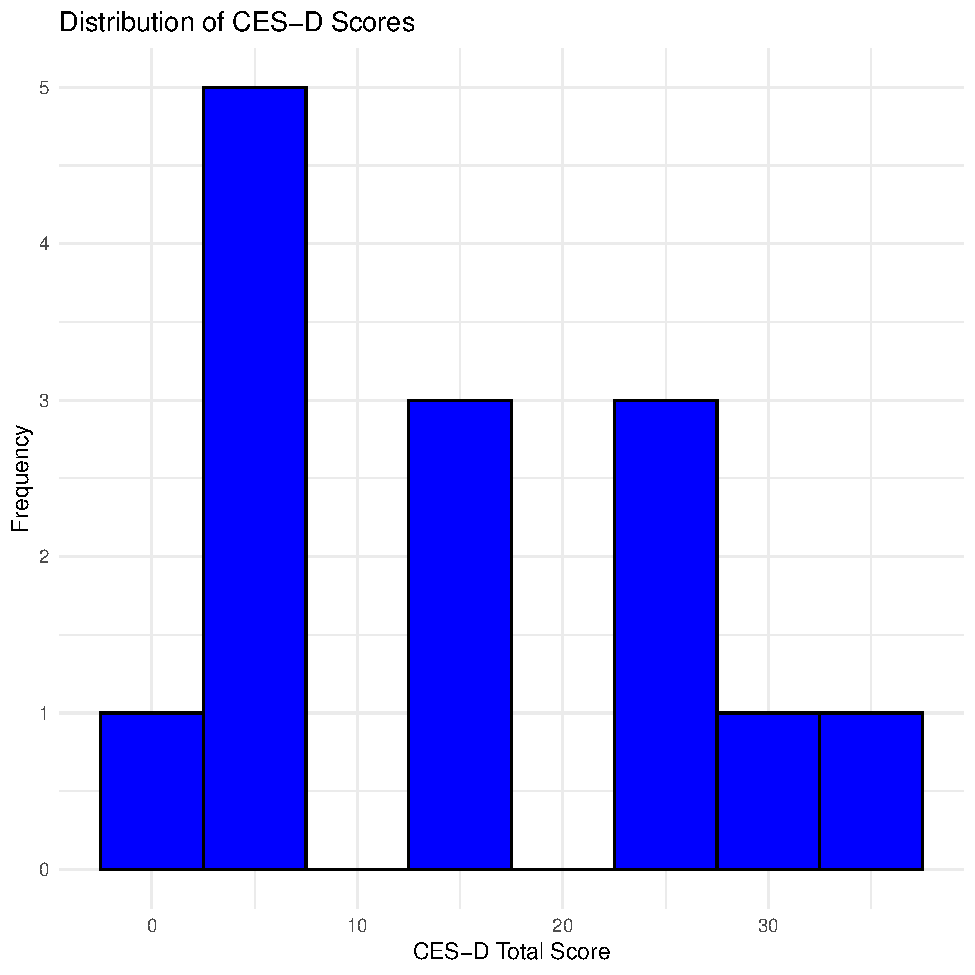
\includegraphics{SE-SCC-Depression_files/figure-pdf/CESD-score-distribution-1.pdf}

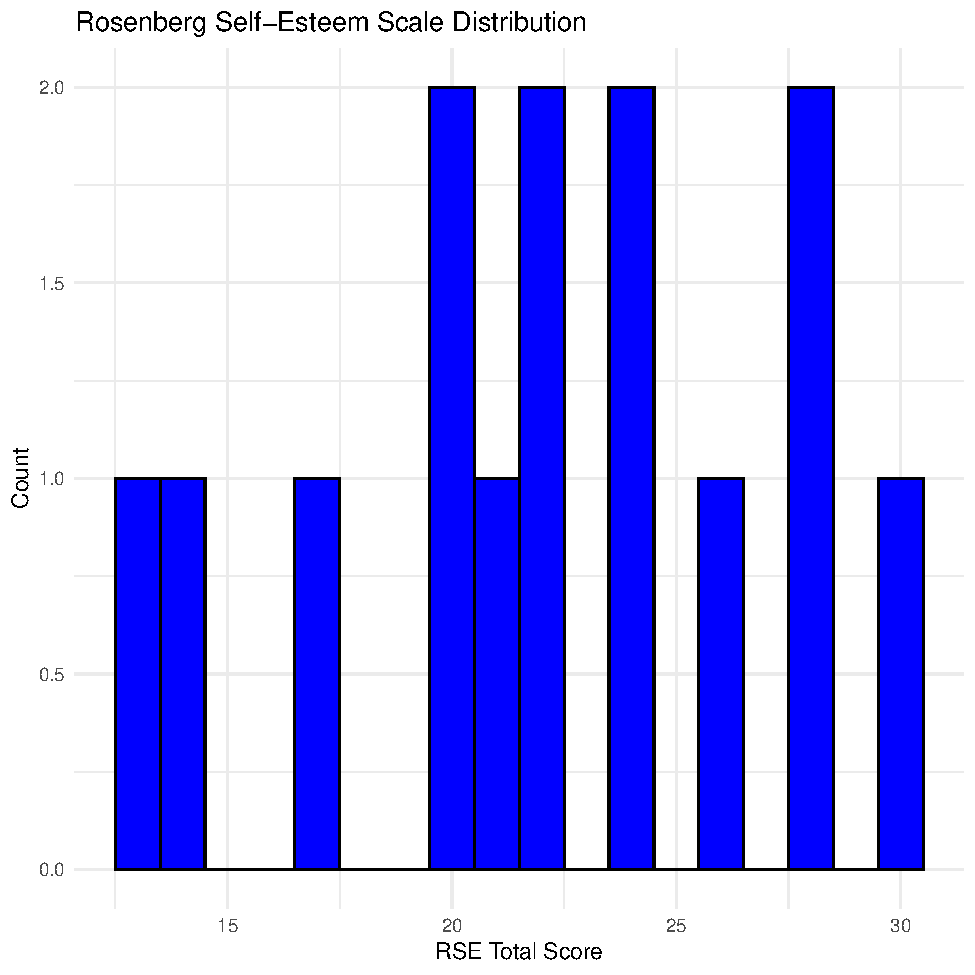
\includegraphics{SE-SCC-Depression_files/figure-pdf/RSES-score-distribution-1.pdf}

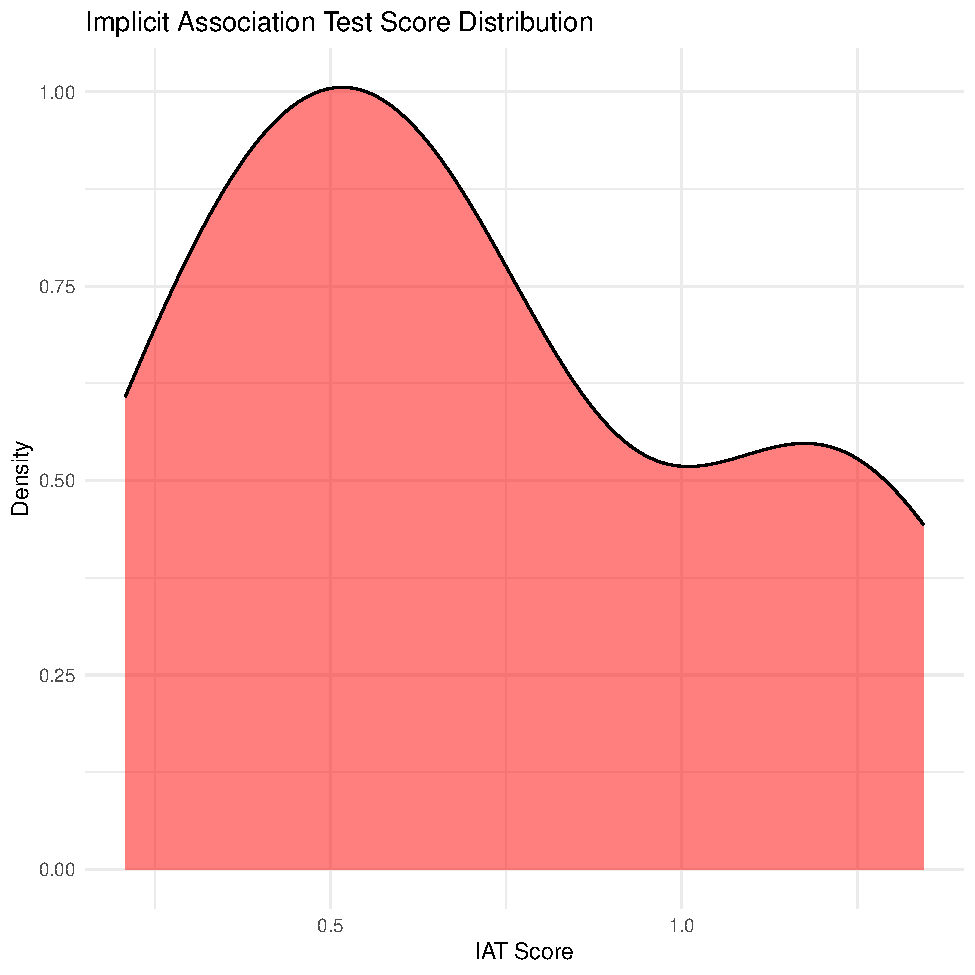
\includegraphics{SE-SCC-Depression_files/figure-pdf/IAT-score-distribution-1.pdf}

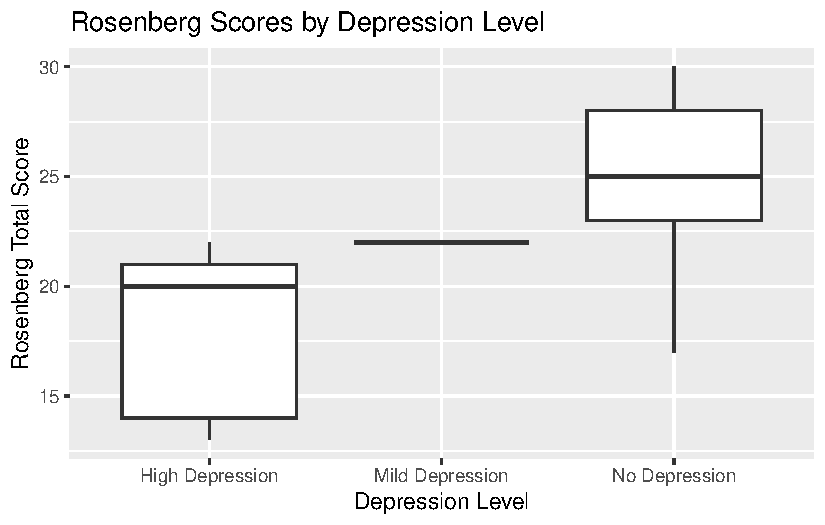
\includegraphics{SE-SCC-Depression_files/figure-pdf/RSES-versus-CESD-level-1.pdf}

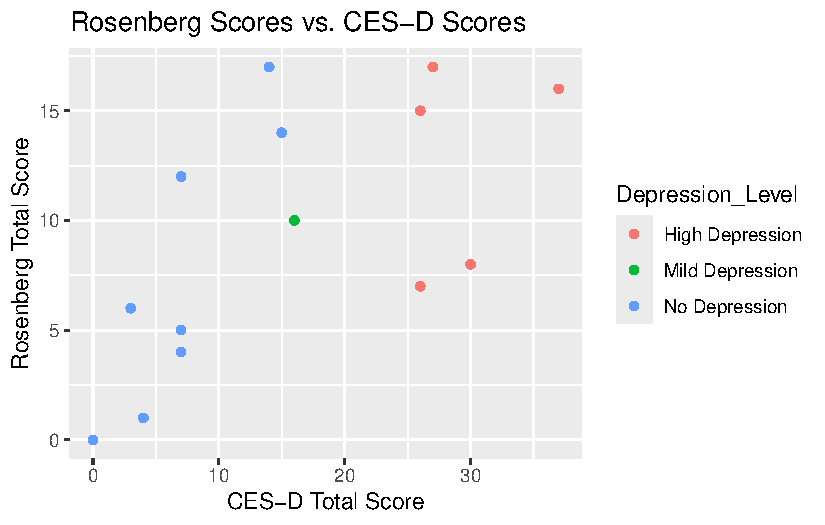
\includegraphics{SE-SCC-Depression_files/figure-pdf/RSES-versus-CESD-total-1.pdf}

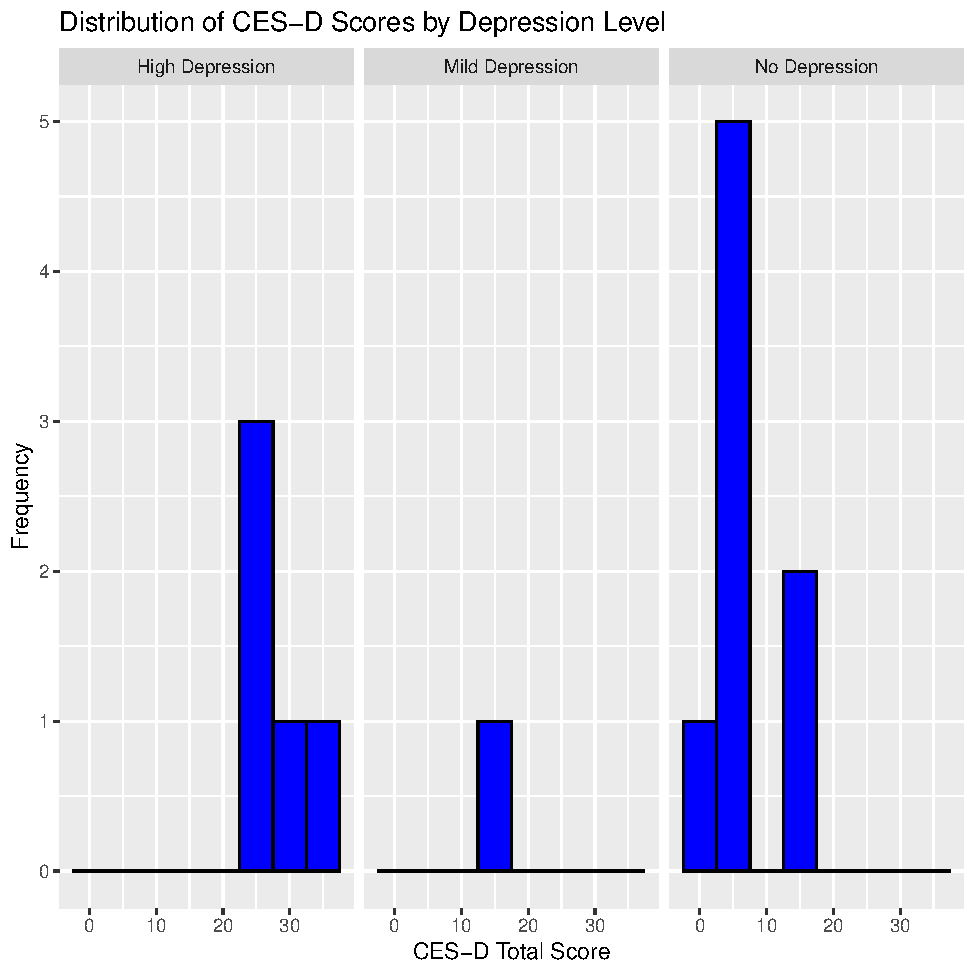
\includegraphics{SE-SCC-Depression_files/figure-pdf/CESD-total-versus-level-1.pdf}

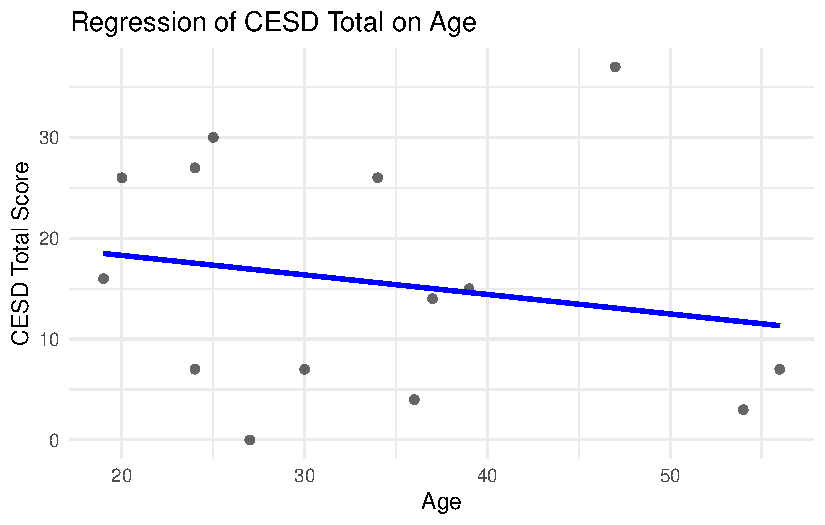
\includegraphics{SE-SCC-Depression_files/figure-pdf/CESD-total-versus-age-1.pdf}

``.

\section{Discussion}\label{discussion}

The results suggest a significant relationship between depression and
self-esteem. There was a mean score of 15.6428571 in the CES-D,
signifying moderate levels of depressive symptoms present in this
sample. In regards to a relationship between age and depressive
symptoms, a linear regression analysis was performed. This demonstrated
that age was not a significant predictor of depression symptoms
(\emph{β} = -0.1935682, \emph{p} = 0.497248). This demonstrates that age
is not significantly predictive of depressive symptoms in this sample.

This cohort measured:

\begin{itemize}
\item
  Depression
\item
  Implicit Self-Esteem
\item
  Explicit Self-Esteem
\end{itemize}

Future cohorts will also measure:

\begin{itemize}
\tightlist
\item
  Self-Concept Clarity
\end{itemize}

\textbf{only use bold to highlight specific data in a table or figure}

\section{References}\label{references}

\phantomsection\label{refs}
\begin{CSLReferences}{1}{0}
\bibitem[\citeproctext]{ref-bhattacharya_effect_2023}
Bhattacharya, S., Kennedy, M., Miguel, C., Tröger, A., Hofmann, S. G.,
\& Cuijpers, P. (2023). Effect of psychotherapy for adult depression on
self-esteem: {A} systematic review and meta-analysis. \emph{Journal of
Affective Disorders}, \emph{325}, 572--581.
\url{https://doi.org/10.1016/j.jad.2023.01.047}

\bibitem[\citeproctext]{ref-butzer_relationships_2006}
Butzer, B., \& Kuiper, N. A. (2006). Relationships between the frequency
of social comparisons and self-concept clarity, intolerance of
uncertainty, anxiety, and depression. \emph{Personality and Individual
Differences}, \emph{41}(1), 167--176.
\url{https://doi.org/10.1016/j.paid.2005.12.017}

\bibitem[\citeproctext]{ref-franck_implicit_2007}
Franck, E., De Raedt, R., Dereu, M., \& Van Den Abbeele, D. (2007).
Implicit and explicit self-esteem in currently depressed individuals
with and without suicidal ideation. \emph{Journal of Behavior Therapy
and Experimental Psychiatry}, \emph{38}(1), 75--85.
\url{https://doi.org/10.1016/j.jbtep.2006.05.003}

\bibitem[\citeproctext]{ref-glashouwer_disorder-specific_2010}
Glashouwer, K. A., \& De Jong, P. J. (2010). Disorder-specific automatic
self-associations in depression and anxiety: Results of {The}
{Netherlands} {Study} of {Depression} and {Anxiety}. \emph{Psychological
Medicine}, \emph{40}(7), 1101--1111.
\url{https://doi.org/10.1017/S0033291709991371}

\bibitem[\citeproctext]{ref-johnson_vulnerability_2016}
Johnson, M., Galambos, N., \& Krahn, H. (2016). Vulnerability, scar, or
reciprocal risk? {Temporal} ordering of self-esteem and depressive
symptoms over 25 years. \emph{Longitudinal and Life Course Studies},
\emph{7}(4). \url{https://doi.org/10.14301/llcs.v7i4.394}

\bibitem[\citeproctext]{ref-rnic_predicting_2023}
Rnic, K. (2023). Predicting recurrence of major depressive episodes
using the {Depression} {Implicit} {Association} {Test}: {A} {Canadian}
biomarker integration network in depression ({CAN}-{BIND}) report.
\emph{Psychiatry Research}.

\bibitem[\citeproctext]{ref-sorjonen_questioning_2022}
Sorjonen, K. (2022). Questioning the vulnerability model: {Prospective}
associations between low self-esteem and subsequent depression ratings
may be spurious. \emph{Journal of Affective Disorders}.

\bibitem[\citeproctext]{ref-visser_beyond_2024}
Visser, L. (2024). \emph{Beyond {Difference} {Scores}: {Unlocking}
{Insights} with {Polynomial} {Regression} in {Studies} on the {Effects}
of {Implicit}-{Explicit} {Congruency}}.

\bibitem[\citeproctext]{ref-yao_electrophysiological_2023}
Yao, J. (n.d.). \emph{Electrophysiological evidence for the
characteristics of implicit self-schema and other-schema in patients
with major depressive disorder: {An} event-related potential study}.

\bibitem[\citeproctext]{ref-yin_relationship_2022}
Yin, X., Shen, J., Jiang, N., Sun, J., Wang, Y., \& Sun, H. (n.d.).
\emph{Relationship of explicit/implicit self‐esteem discrepancies,
suicide ideation, and suicide risk in patients with major depressive
disorder}.

\end{CSLReferences}






\end{document}
